\let\negmedspace\undefined
\let\negthickspace\undefined
\documentclass[journal]{IEEEtran}
\usepackage[a5paper, margin=10mm, onecolumn]{geometry}
\usepackage{lmodern} % Ensure lmodern is loaded for pdflatex
\usepackage{tfrupee} % Include tfrupee package

\setlength{\headheight}{1cm} % Set the height of the header box
\setlength{\headsep}{0mm}     % Set the distance between the header box and the top of the text

\usepackage{gvv-book}
\usepackage{gvv}
\usepackage{cite}
\usepackage{amsmath,amssymb,amsfonts,amsthm}
\usepackage{algorithmic}
\usepackage{graphicx}
\usepackage{textcomp}
\usepackage{xcolor}
\usepackage{txfonts}
\usepackage{listings}
\usepackage{enumitem}
\usepackage{mathtools}
\usepackage{gensymb}
\usepackage{comment}
\usepackage[breaklinks=true]{hyperref}
\usepackage{tkz-euclide} 
\usepackage{listings}
\def\inputGnumericTable{}                                 
\usepackage[latin1]{inputenc}                                
\usepackage{color}                                            
\usepackage{array}                                            
\usepackage{longtable}                                       
\usepackage{calc}                                             
\usepackage{multirow}                                         
\usepackage{hhline}                                           
\usepackage{ifthen}                                           
\usepackage{lscape}

\begin{document}
	
	\bibliographystyle{IEEEtran}
	\vspace{3cm}
	
	\title{12.6.6.8}
	\author{EE24BTECH11030 - KEDARANANDA}
	% \maketitle
	% \newpage
	% \bigskip
	{\let\newpage\relax\maketitle}
	
	\renewcommand{\thefigure}{\theenumi}
	\renewcommand{\thetable}{\theenumi}
	\setlength{\intextsep}{10pt} % Space between text and floats
	\textbf{Question:}
	Find the maximum area of an isosceles triangle inscribed in the ellipse $\frac{x^2}{a^2}+\frac{y^2}{b^2}=1$with its vertex at one end of the major axis.\\
	\textbf{Solution:}
	
	\textbf{Theoretical solution:}
	Consider the isosceles triangle ABC: \\
	$A(a, 0)$, $B(a \cos\theta, b \sin\theta)$, and $C(a \cos\theta, -b \sin\theta)$ \\
	
	\begin{align}
		\text{Area of } \triangle ABC &= \frac{1}{2} \times BC \times \text{height of } \triangle ABC \\
		\text{Height of } \triangle ABC &= a(1 - \cos\theta) \\
		BC &= 2b \sin\theta \\
		\Delta &= \frac{1}{2} \times 2b \sin\theta \times a(1 - \cos\theta) \\
		&= ab \sin\theta (1 - \cos\theta)
	\end{align}
	
	For the maximum area of the triangle:
	\begin{align}
		\frac{d\Delta}{d\theta} = ab \cos\theta (1 - \cos\theta) + ab \sin^2\theta = 0 \\
		\cos\theta (1 - \cos\theta) + \sin^2\theta = 0 \\
		\cos\theta=\cos{2\theta}\\
	\end{align}
	
	\begin{align}
		\cos\theta = -\frac{1}{2} \\
	\end{align}
	
	For the maximum value:
	\begin{align}
		\cos\theta &= -\frac{1}{2}, \quad \sin\theta = \frac{\sqrt{3}}{2} \\
		\text{Maximum area} &= ab \times \frac{\sqrt{3}}{2} \left( 1 + \frac{1}{2} \right) \\
		&= \frac{3\sqrt{3}}{4} ab
	\end{align}
	\textbf{Computational solution:}
	\newline
	By the gradient descent algorithm, the difference equation is given by,
	\begin{align}
		f(x)=ab \sin{x} (1 - \cos{x})\\
	\end{align}
	to find value of $x_n$ for max area\\
	\begin{align}
		x_{n + 1} = x_n + \mu f^{\prime}\brak{x_{n}}\\
		x_{n + 1} = x_n + \mu \brak{ab \cos{x_{n}} (1 - \cos{x_{n}}) + ab \sin^2{x_{n}}}
	\end{align}
	\[
	x_{n+1} = x_n + \mu ab \cos x_n (1 - \cos x_n) + \mu ab \sin^2 x_n
	\]
	Taking the Z-transform on both sides:
	\[
	zX(z) - zx_0 = X(z) + \mu ab \cos(X(z))(1 - \cos(X(z))) + \mu ab \sin^2(X(z)).
	\]
	\begin{align}
		(Z-1)X(Z)-Zx_{0}={\mu}ab\left(\frac{1-Z^{-1}\cos{1}}{1-2Z^{-1}\cos{1}+Z^{-2}}-\frac{1-Z^{-1}\cos{2}}{1-Z^{-1}\cos{2}+Z^{-2}}\right)
	\end{align}
	If the sequence $x_n$ has to converge,
	\begin{align}
		\lim_{n\to\infty} \abs{x_{n + 1} - x_n} &= 0\\
		\implies \lim_{n\to\infty} \abs{{\mu}ab(\cos(2x_{n})-\cos(x_{n}))} &= 0\\
		\implies \mu \lim_{n\to\infty} \abs{{\mu}ab(\cos(2x_{n})-\cos(x_{n}))} &= 0 \text{, } \mu > 0\\
		\implies \lim_{n\to\infty} \cos(2x_{n})-\cos(x_{n}) = 0\\
		\implies \lim_{n\to\infty} x_{n} = \frac{2\pi}{3}
	\end{align}
	to find value of $x_n$ for min area\\
	\begin{align}
		x_{n + 1} = x_n - \mu f^{\prime}\brak{x_{n}}\\
		x_{n + 1} = x_n - \mu \brak{ab \cos{x_{n}} (1 - \cos{x_{n}}) + ab \sin^2{x_{n}}}
	\end{align}
	\[
	x_{n+1} = x_n - \mu ab \cos x_n (1 - \cos x_n) + \mu ab \sin^2 x_n
	\]
	Taking the Z-transform on both sides:
	\[
	zX(z) - zx_0 = X(z) - \mu ab \cos(X(z))(1 - \cos(X(z))) + \mu ab \sin^2(X(z)).
	\]
	\begin{align}
		(Z-1)X(Z)-Zx_{0}=-{\mu}ab\left(\frac{1-Z^{-1}\cos{1}}{1-2Z^{-1}\cos{1}+Z^{-2}}-\frac{1-Z^{-1}\cos{2}}{1-Z^{-1}\cos{2}+Z^{-2}}\right)
	\end{align}
	If the sequence $x_n$ has to converge,
	\begin{align}
		\lim_{n\to\infty} \abs{x_{n + 1} - x_n} &= 0\\
		\implies \lim_{n\to\infty} \abs{-{\mu}ab(\cos(2x_{n})-\cos(x_{n}))} &= 0\\
		\implies \mu \lim_{n\to\infty} \abs{-{\mu}ab(\cos(2x_{n})-\cos(x_{n}))} &= 0 \text{, } \mu > 0\\
		\implies \lim_{n\to\infty} \cos(2x_{n})-\cos(x_{n}) = 0\\
		\implies \lim_{n\to\infty} x_{n} = 0
	\end{align}
	\begin{figure}[h!]
		\centering
		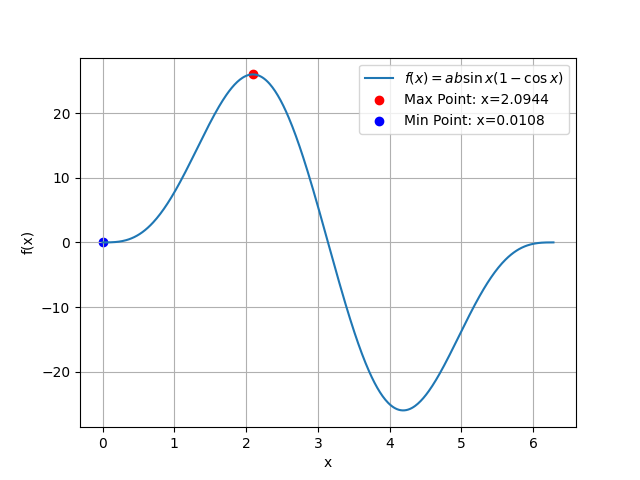
\includegraphics[width=0.7\columnwidth]{figs/Fig1.png}
		\label{label}
	\end{figure}
	
\end{document}